\section{API Documentation}\label{sec:api_documentation}
As mentioned in \cref{cha:requirements_elicitation} our development focus is on the server, resulting in our users being developers; since the server is to be used by other systems.
As a result our API documentation becomes the interface with which developers interact.
How the API documentation is created is described in \cref{sec:services_overview}, in this section we describe provide an example of the documentation.

\bigskip
Developers for a client, be it producer or consumer, may have no insight into how the server is organised, however, they will be in possesion of the API documentation.
The API documentation accurately describes which endpoints exists, which requests can be made, what paramaters a request requires, and provides an example of both a request and a response.
As mentioned in \cref{sec:services_overview} we use Javadocs in combination with Enunciate to produce the API documenation, an example of the output is shown on \cref{fig:enunciate_example}.

\begin{figure}[!htb]
    \centering
    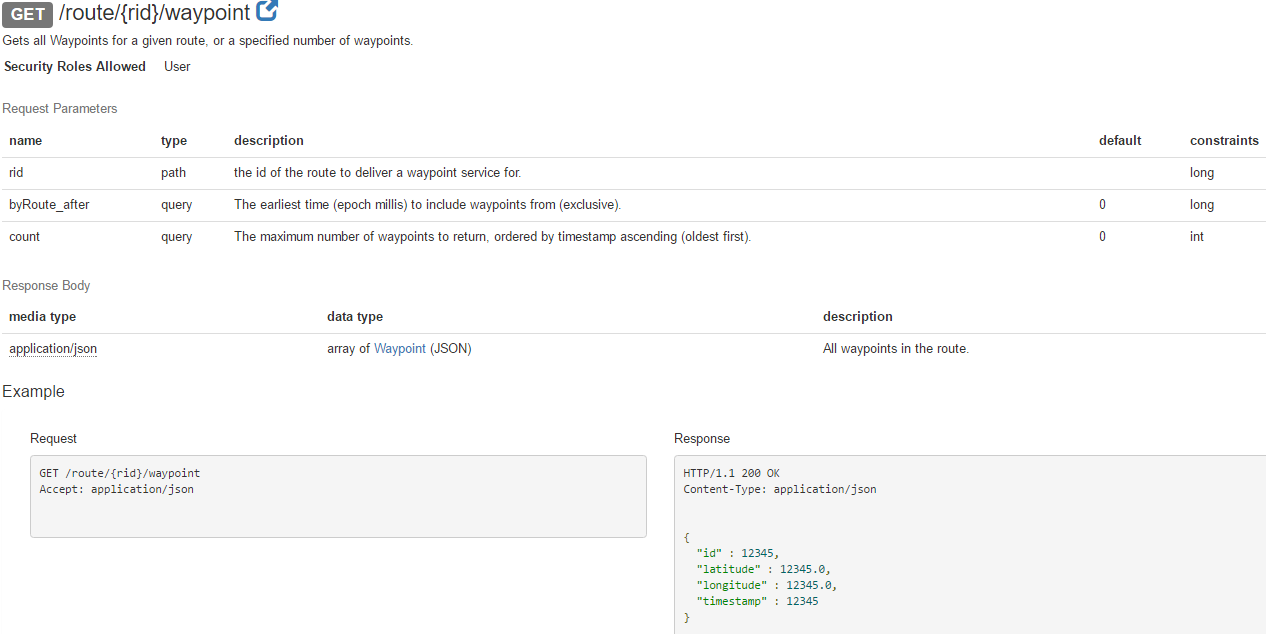
\includegraphics[width=1\textwidth]{img/cuckcuckcuckcuck.png}
    \caption{API Documentation created by Enunciatte for the get request of a waypoint.}
    \label{fig:enunciate_example}
\end{figure}
